\documentclass[12pt,a4paper]{article}

\usepackage[utf8]{inputenc}
\usepackage[T1]{fontenc}
\usepackage{lmodern}
\usepackage[english]{babel}
\usepackage[margin=2.5cm]{geometry}
\usepackage{graphicx}
\usepackage{booktabs}
\usepackage{tabularx}
\usepackage{array}
\usepackage{listings}
\usepackage{xcolor}
\usepackage{fancyhdr}
\usepackage{tcolorbox}
\usepackage{enumitem}
\usepackage{microtype}
\usepackage{caption}
\usepackage{hyperref}

\definecolor{primary}{RGB}{18,52,86}
\definecolor{secondary}{RGB}{41,128,185}
\definecolor{codebg}{RGB}{247,249,250}
\definecolor{codeframe}{RGB}{209,213,219}
\definecolor{codegreen}{RGB}{39,136,60}
\definecolor{codegray}{RGB}{108,117,125}

\hypersetup{colorlinks=true,linkcolor=primary,urlcolor=secondary,citecolor=secondary}

\lstdefinestyle{code}{
    backgroundcolor=\color{codebg}, basicstyle=\small\ttfamily,
    keywordstyle=\color{secondary}\bfseries, stringstyle=\color{codegreen},
    commentstyle=\color{codegray}\itshape, numbers=left,
    numberstyle=\tiny\color{codegray}, numbersep=8pt, frame=single,
    rulecolor=\color{codeframe}, breaklines=true, breakatwhitespace=true,
    showstringspaces=false, tabsize=4, captionpos=b
}
\lstdefinestyle{plain}{
    backgroundcolor=\color{codebg}, basicstyle=\small\ttfamily,
    frame=single, rulecolor=\color{codeframe}, breaklines=true,
    showstringspaces=false, captionpos=b
}
\lstdefinestyle{term}{
    backgroundcolor=\color{black}, basicstyle=\small\ttfamily\color{white},
    frame=none, numbers=none, breaklines=true, showstringspaces=false,
    captionpos=b
}

\pagestyle{fancy}
\fancyhf{}
\fancyhead[L]{\small Network Programming --- Laboratory Work 3}
\fancyhead[R]{\small Dinu Plesu, FAF-241}
\fancyfoot[C]{\thepage}
\renewcommand{\headrulewidth}{0.4pt}
\renewcommand{\footrulewidth}{0pt}

\newcommand{\studentgroup}{FAF-241}

\begin{document}
\sloppy
\setlength{\emergencystretch}{3em}

\begin{titlepage}
    \centering
    {\large \textbf{TECHNICAL UNIVERSITY OF MOLDOVA}}\\[0.2cm]
    {\large Faculty of Computers, Informatics and Microelectronics}\\[0.2cm]
    {\large Department of Software Engineering and Automatics}\\[0.8cm]

    
\includegraphics[width=3.5cm]{figures/utm_logo.png}\\[1.2cm]

    {\Large \textbf{LABORATORY WORK NO. 3}}\\[0.4cm]
    {\LARGE \textbf{A Local Network Chat:\\ UDP Sockets, Broadcast Discovery, and Encrypted Private Messages}}\\[0.4cm]
    {\large Course: Network Programming}\\[2.5cm]

    \begin{minipage}{0.45\textwidth}
        \flushleft
        \textbf{Author:}\\
        Dinu \textsc{Plesu}\\
        Student of group: \studentgroup
    \end{minipage}
    \hfill
    \begin{minipage}{0.45\textwidth}
        \flushright
        \textbf{Verified by:}\\
        Lecturer / Supervisor\\
        Fistic Cristofor
    \end{minipage}

    \vfill
    {\large Chi\c{s}in\u{a}u --- 2026}
\end{titlepage}

\newpage
\tableofcontents
\newpage

\section{Introduction}

The goal of this laboratory work is to build a chat for the local network using
UDP sockets directly. There is no server: every running copy of the program is a
peer that both sends and receives. A message for the general channel reaches
everybody with one datagram; a private message goes to one peer only; the last
task encrypts private messages so that nobody outside the chat can read them.

The implementation is written twice, in C\# and in Go, and the two programs
interoperate. The C\# peer uses the \texttt{Socket} class with
\texttt{SocketType.Dgram}; the Go peer uses \texttt{net.UDPConn}. No
\texttt{UdpClient}, no chat or service-discovery library, and no messaging
framework is used.

The report describes the protocol, the two-socket design, discovery and
keep-alive, private messages, encryption, and the two-desktop verification run
made on 26 November 2026. In that run two Go peers ran on a CachyOS desktop and
one C\# peer ran on a Windows desktop, all on the same Wi-Fi network, with three
peers on two computers. A second local test exercised a duplicate name and
invalid/oversized datagrams.

\section{Architecture and protocol}

\subsection{One program, two sockets}

Every peer creates two UDP sockets:

\begin{itemize}[itemsep=2pt]
    \item \textbf{general socket}: bound to \texttt{0.0.0.0:<chatPort>}, with
          address/port reuse so that several peers can share the port on one
          computer. It sends and receives the general channel and the discovery
          messages.
    \item \textbf{private socket}: bound to \texttt{0.0.0.0:0}, which gives a
          unique ephemeral port. It receives private messages addressed to this
          peer only.
\end{itemize}

The private endpoint (local IP and ephemeral port) is advertised in
\texttt{join}, \texttt{hello} and \texttt{heartbeat}. A peer never sends a
private message to the shared chat port, because a unicast datagram to a port
shared by several sockets reaches only one of them.

\subsection{Datagrams}

Every message is one UDP datagram containing one JSON object. Table
\ref{tab:messages} lists the message types.

\begin{table}[h]
\centering
\small
\begin{tabularx}{\textwidth}{@{}l l X@{}}
\toprule
Type & Direction & Meaning \\
\midrule
\texttt{join} & broadcast & a new peer announces its name and private endpoint \\
\texttt{hello} & broadcast & an existing peer answers a join \\
\texttt{heartbeat} & broadcast & ``I am still here'', every 5 s \\
\texttt{bye} & broadcast & the peer leaves with \texttt{/quit} \\
\texttt{gen} & broadcast & one general-channel message \\
\texttt{priv} & unicast & one private message (no passphrase) \\
\texttt{privenc} & unicast & one encrypted private message \\
\texttt{nameinuse} & unicast & the name is already taken; the newcomer exits \\
\bottomrule
\end{tabularx}
\caption{Message types of the chat protocol.}
\label{tab:messages}
\end{table}

A general message carries \texttt{from}, \texttt{text} and a per-peer
\texttt{id}. A private encrypted message carries \texttt{from}, \texttt{to},
the base64 nonce, tag and ciphertext.

\subsection{General channel and discovery}

A line that does not start with a slash is sent as one \texttt{gen} datagram.
The datagram is sent to every directed broadcast address of the computer (for
example \texttt{192.168.1.255}), to the limited broadcast
\texttt{255.255.255.255}, and to the loopback broadcast
\texttt{127.255.255.255}. The first two reach the other computers; the last one
reaches the other peers on the same computer, because a broadcast sent out the
network card does not come back to local sockets.

The author also receives its own datagram. The peer ignores a \texttt{gen} whose
\texttt{from} is its own name, and deduplicates the other copies with the
\texttt{from:id} key, so a message is shown exactly once.

When a peer starts, it broadcasts \texttt{join}. Every online peer adds it,
answers with \texttt{hello} and the newcomer learns the complete list within
about one second. Heartbeats are sent every 5 seconds; a peer that has not been
heard for 15 seconds is removed and shown as left. \texttt{/quit} broadcasts
\texttt{bye} immediately.

Names are unique. If a peer receives a \texttt{join} with its own name but a
different endpoint, it sends \texttt{nameinuse} to that endpoint. The newcomer
prints an error and exits; it never joins.

\subsection{Private messages}

\texttt{/msg name text} looks the receiver up in the peer table and sends one
datagram to its private endpoint. The sender prints
\texttt{[private] you -> name: text}; the receiver prints
\texttt{[private] name: text}. A message to a name that is not online produces
an error.

A peer may advertise the wrong interface in its private endpoint when the
computer has several network cards. The receiver therefore keeps the advertised
private port but takes the IP address from the UDP datagram source. This makes
private messages work on the real LAN address even when the sender is
multi-homed.

\subsection{Encryption}

All peers of a chat receive the same passphrase as a command-line parameter.
Each peer derives a 32-byte key with PBKDF2-HMAC-SHA256, 100\,000 iterations
and a 16-byte zero salt. Every private message uses AES-256-GCM with a fresh
random 12-byte nonce from the OS CSPRNG. The nonce, the 16-byte authentication
tag and the ciphertext are sent base64-encoded in the JSON datagram. The
receiver decrypts and authenticates the message; a wrong passphrase or a
modified ciphertext fails the GCM check and the message is dropped.

The general channel is not encrypted, as the task specifies.

\subsection{Logging and invalid input}

Every peer writes \texttt{chat-<name>-<port>.log} with one line for every
datagram it sends, receives or drops: time, direction, endpoint, kind and size.
The log is the evidence for the defense.

The receive loops validate every datagram. Non-JSON bytes, an unknown type, a
general message longer than 500 characters, and a datagram larger than 2000
bytes are logged as \texttt{DROP} and ignored. The chat never crashes because of
a datagram from another program.

\section{Implementation}

\subsection{C\# peer}

The C\# peer uses two \texttt{Socket} objects, one bound to
\texttt{IPAddress.Any} and the chat port with \texttt{ReuseAddress}, and one
bound to an ephemeral port. The receive loops run on separate threads so that
incoming messages are printed while the user types. A console writer lock
prevents two threads from interleaving output. On Windows the peer also
disables \texttt{SIO\_UDP\_CONNRESET}: without it, an ICMP port-unreachable from
a peer that just left would make the next receive fail with ``connection
forcibly closed''.

\subsection{Go peer}

The Go peer uses \texttt{net.ListenConfig} with a control function that sets
\texttt{SO\_REUSEADDR}, \texttt{SO\_BROADCAST} and, on Unix,
\texttt{SO\_REUSEPORT}. Receiving runs in two goroutines; a mutex protects the
peer table and the seen-message set. The binary is built with the standard
library only (no third-party modules).

\subsection{The local-peer broadcast fix}

The first two-desktop run used port 9000. Both Go peers on the Linux desktop
could send, and the Windows peer received their datagrams, but the two local Go
peers did not receive each other and the Linux peers did not receive the
Windows broadcasts. Two separate causes were found:

\begin{enumerate}[itemsep=2pt]
    \item A broadcast sent out the Wi-Fi card is not delivered back to the
          other local sockets. The fix is the extra \texttt{127.255.255.255}
          target; a small Go test bound two sockets to the same port and showed
          that both receive the loopback broadcast, while they do not receive
          the \texttt{192.168.1.255} copy.
    \item The Linux desktop runs UFW with the default input policy \texttt{DROP}.
          Port 9000/UDP was not allowed, so the Windows broadcasts never
          reached the Linux peers. The second run used port 25565/UDP, which
          the existing UFW rules already allow. The task allows any chat port;
          all peers used the same one.
\end{enumerate}

After the fix, all three peers discovered each other, the two local peers
received the general channel, and the Windows peer exchanged encrypted private
messages with both Linux peers.

\section{Testing and results}

\subsection{Environment}

\begin{table}[h]
\centering
\small
\begin{tabularx}{\textwidth}{@{}l X@{}}
\toprule
Component & Value used for the measurements \\
\midrule
Desktop A (Windows) & HP OMEN, Intel Core i5-13420H, 8 cores / 12 threads, 16 GB RAM, Windows 11 IoT Enterprise LTSC 10.0.26300, .NET 10 \\
Desktop B (Linux) & CachyOS, Linux 7.3.6-1, Intel Core i5-10300H, 4 cores / 8 threads, 7.6 GiB RAM, Go 1.27.4 \\
Network & same Wi-Fi subnet, 192.168.1.0/24; A = 192.168.1.41, B = 192.168.1.22 \\
Chat port & 25565/UDP (same on all peers) \\
Passphrase & \texttt{secret} \\
\bottomrule
\end{tabularx}
\caption{Two-desktop test environment.}
\end{table}

The peers were: \textbf{Cara} (C\#, Windows), \textbf{Alice} and \textbf{Bob}
(Go, Linux). Alice and Bob ran on the same computer and shared port 25565; the
third peer ran on the other computer. This exercises both requirements at once:
several peers on one computer, and at least three peers on at least two
computers.

\subsection{Discovery and the general channel}

All three peers discovered each other within about a second. The console output
of Alice is shown in Listing~\ref{lst:alice}; Bob and Cara show the same three
participants. Each general message from each peer appears once on every peer,
including its author.

\begin{lstlisting}[style=term,caption={Alice (Linux, Go): discovery, general channel, users and encrypted private messages.},label={lst:alice}]
* Bob joined the chat
* Cara joined the chat
* Alice joined (private ep 192.168.1.22:59308). Type messages, /msg name text, /users, /quit
[general] Cara: hello from Cara on windows
[general] Bob: hello from Bob on linux
[general] Alice: hello from Alice on linux
Online:
  Bob 192.168.1.22:50827
  Cara 192.168.1.41:52413
[private] you -> Bob: private from Alice
[private] you -> Cara: private from Alice
[private] Bob: private from Bob
* Cara left the chat
\end{lstlisting}

\subsection{Private messages and encryption}

Four private messages were exchanged: Alice to Bob, Alice to Cara, Bob to Cara
and Bob to Alice. The receiver's console shows only the messages addressed to
it. Listing~\ref{lst:bob} shows Bob receiving the two messages addressed to him
and sending two; Cara never sees Alice--Bob traffic.

\begin{lstlisting}[style=term,caption={Bob (Linux, Go): only the private messages addressed to Bob are shown.},label={lst:bob}]
* Alice joined the chat
* Cara joined the chat
* Bob joined (private ep 192.168.1.22:50827). Type messages, /msg name text, /users, /quit
[general] Cara: hello from Cara on windows
[general] Alice: hello from Alice on linux
[general] Bob: hello from Bob on linux
Online:
  Alice 192.168.1.22:59308
  Cara 192.168.1.41:52413
[private] you -> Cara: private from Bob
[private] Alice: private from Alice
[private] you -> Alice: private from Bob
* Cara left the chat
\end{lstlisting}

The datagram log confirms the encryption on the wire. Listing~\ref{lst:log}
shows Cara sending an encrypted private datagram to Bob's private endpoint and
receiving the encrypted replies from both Linux peers. The payload is
\texttt{privenc}, not the plaintext.

\begin{lstlisting}[style=plain,caption={Excerpt from Cara's datagram log: encrypted private traffic.},label={lst:log}]
... SEND 192.168.1.22:50827 privenc 137
... RECV 192.168.1.22:50827 private 132
... RECV 192.168.1.22:59308 private 134
\end{lstlisting}

\subsection{Users, leave, duplicate names and invalid input}

\texttt{/users} listed all three peers on all three consoles. \texttt{/quit}
broadcast \texttt{bye}; the remaining peers printed
\texttt{* Cara left the chat}.

A second peer started with the name \texttt{Alice} while Alice was online. It
received \texttt{nameinuse} and exited:

\begin{lstlisting}[style=term]
ERROR: name 'Alice' already in use
\end{lstlisting}

Three invalid datagrams were sent to a peer from the other computer: 14 random
bytes, a JSON \texttt{gen} with a 600-character text, and a 3000-byte datagram.
The peer logged and dropped them without crashing:

\begin{lstlisting}[style=plain]
... RECV 192.168.1.41:49918 general 14
... DROP 192.168.1.41:49918 invalid_json 14
... RECV 192.168.1.41:49918 general 652
... DROP 192.168.1.41:49918 gen_too_long 652
... RECV 192.168.1.41:49918 general 3000
... DROP 192.168.1.41:49918 too_long 3000
\end{lstlisting}

\begin{figure}[h]
\centering
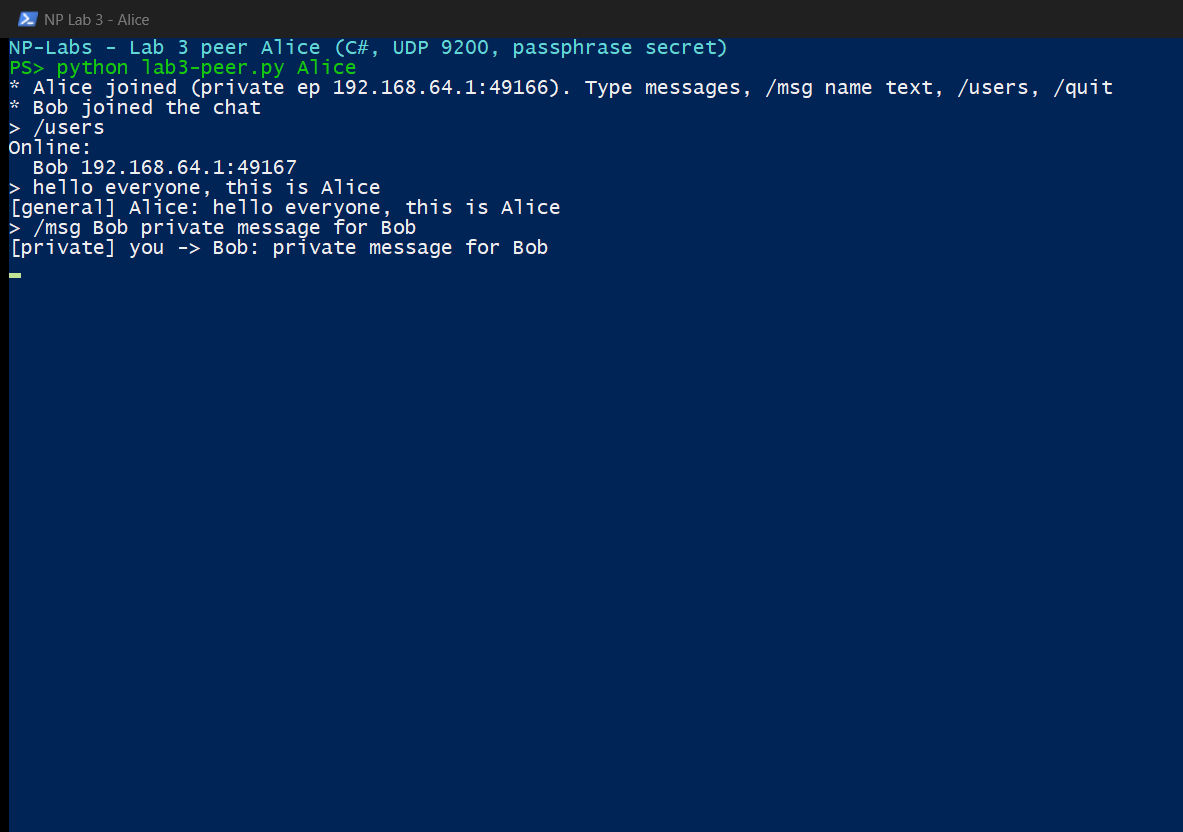
\includegraphics[width=0.9\linewidth]{figures/lab3-alice.png}
\caption{A peer console: discovery, general channel and private message.}
\label{fig:alice}
\end{figure}

\begin{figure}[h]
\centering
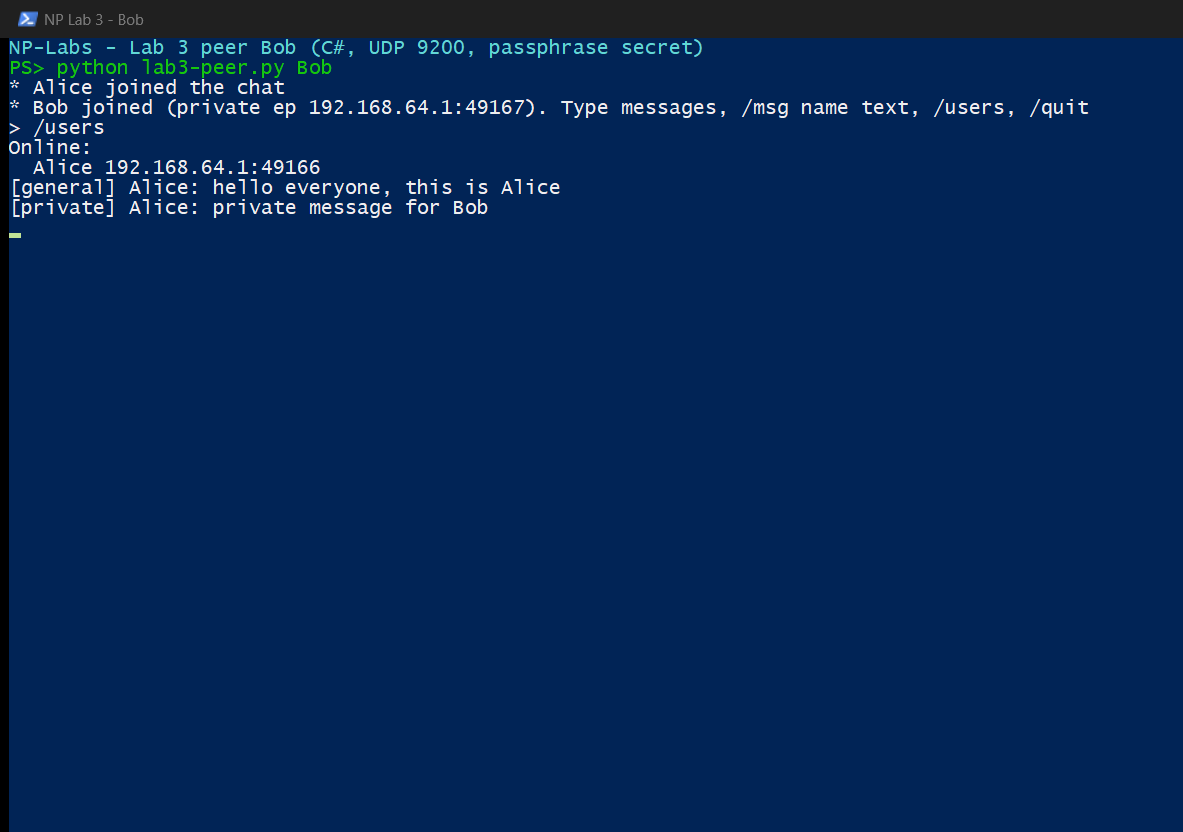
\includegraphics[width=0.9\linewidth]{figures/lab3-bob.png}
\caption{The other peer sees only the private message addressed to it.}
\label{fig:bob}
\end{figure}

\subsection{Summary of checks}

\begin{table}[h]
\centering
\small
\begin{tabularx}{\textwidth}{@{}X l@{}}
\toprule
Check & Result \\
\midrule
Three peers on two computers discover each other & pass \\
Two peers share one port on the Linux computer & pass \\
General message from each peer reaches all, once & pass \\
Private message reaches only its receiver & pass \\
Private messages are AES-GCM encrypted on the wire & pass \\
\texttt{/users} lists all online peers & pass \\
\texttt{/quit} produces a leave notice & pass \\
Duplicate name is refused and the newcomer exits & pass \\
Invalid, oversized and too-long datagrams are dropped & pass \\
C\# and Go peers interoperate (general and encrypted private) & pass \\
\bottomrule
\end{tabularx}
\caption{Results of the two-desktop Lab 3 run.}
\end{table}

\section{Answers to the defense questions}

\subsection*{Task 1}

\textbf{1. Why bind 0.0.0.0 and not the IP or 127.0.0.1?}
\texttt{0.0.0.0} receives on every interface, so the chat works on Wi-Fi,
Ethernet, hotspot or USB tethering without knowing the address in advance. A
specific IP binds only that interface; \texttt{127.0.0.1} sees only the same
machine.

\textbf{2. How can several peers on one computer bind the same port? Which receive a general message?}
\texttt{SO\_REUSEADDR} and \texttt{SO\_REUSEPORT} let several UDP sockets bind
the same address and port. A broadcast or multicast datagram is delivered to
all of them, so every local peer sees the general channel. A unicast to that
shared port is delivered to only one socket, which is why private messages use
a separate unique port.

\textbf{3. Your own message comes back; how is it recognized?}
The datagram carries \texttt{from} and an \texttt{id}. A peer ignores datagrams
whose \texttt{from} is its own name (it already printed the message locally),
and deduplicates \texttt{from:id} because the general message is sent to
several broadcast addresses.

\textbf{4. Why at most 500 characters? What would happen at 100,000?}
The maximum IPv4 UDP payload is 65,507 bytes, but real networks fragment above
the MTU (about 1,400 safe bytes), and one lost fragment loses the datagram. 500
UTF-8 characters stay well below that. 100,000 characters would exceed the
datagram limit, fail to send or be fragmented and dropped; the receiver also
drops anything over 500 characters.

\subsection*{Task 2}

\textbf{1. How does a new peer learn who is online, and how long does it take?}
It broadcasts \texttt{join} with its name and private endpoint. Every online
peer adds it, replies with \texttt{hello}, and the newcomer waits about 1.2 s;
the list is complete within about a second.

\textbf{2. A peer process is killed. How and when do the others notice? Why not at once?}
UDP has no connection and no FIN/RST. Peers send \texttt{heartbeat} every 5 s
and remove a peer whose last heartbeat is older than 15 s. A killed process is
noticed after up to about 15 s. TCP would notice a closed connection at once
because the kernel sends FIN/RST.

\textbf{3. Two peers start with the same name at the same moment. What happens?}
Both broadcast \texttt{join}. Each sees a \texttt{join} with its own name but a
different private endpoint, sends \texttt{nameinuse} to that endpoint, and
exits. In practice at least one is rejected; the survivor keeps the name. The
check is \texttt{name == my name \&\& endpoint != my endpoint}, so a peer's own
loopback is not mistaken for a conflict.

\subsection*{Task 3}

\textbf{1. Several peers on one computer share the chat port. How does a private message reach the right one?}
Every peer also binds a second socket to an ephemeral port and advertises that
endpoint. A private message is sent to that unique endpoint, not to the shared
chat port, so only the intended peer receives it, even on the same machine.

\textbf{2. Why not send a private message to everybody with the receiver name inside?}
Everyone would receive and could read it; it also wastes bandwidth and breaks
the privacy requirement.

\textbf{3. What happens to a private message sent to a peer that left a second ago?}
The sender's list may still contain it until the 15 s timeout. The datagram goes
to a closed port and is lost; UDP has no delivery confirmation.

\textbf{4. UDP can lose a private message. How could the sender know, and what would it do?}
Add an application-level ACK: the receiver sends \texttt{ack(id)}, the sender
retries with a timeout and a retry limit; or use TCP. This lab does not
implement ACKs, so a lost private message is lost.

\subsection*{Task 4}

\textbf{1. Why derive the key with a KDF instead of using the passphrase bytes?}
A passphrase is low-entropy and has arbitrary length. PBKDF2 stretches it with
100,000 iterations to a fixed 32-byte key and makes brute-force guessing slower.

\textbf{2. Which algorithm encrypts messages? Why must the nonce never repeat? Where do yours come from?}
AES-256-GCM. Reusing a nonce with the same key breaks GCM's confidentiality and
authentication guarantees. Each message uses a fresh random 12-byte nonce from
a CSPRNG; the nonce is sent with the ciphertext and tag.

\textbf{3. Every member knows the passphrase. Who can read Ana--Ion? What would be needed for only the two?}
Any member who knows the passphrase can derive the key and read every private
message. To restrict it to Ana and Ion, they would need a per-pair key exchange
(for example authenticated Diffie--Hellman) and encryption with that pair key,
not a chat-wide key.

\textbf{4. Can someone without the passphrase change an encrypted message unnoticed? What protects it?}
No. AES-GCM produces an authentication tag over the ciphertext; any change
makes the decryption fail, and the receiver logs a decryption failure and drops
the message. Without the key the attacker cannot forge a valid tag.

\subsection*{Control questions}

\textbf{1. Which TCP promises does UDP not make?} Connection setup, reliable
delivery, ordering, no duplication, flow/congestion control and stream
semantics. The chat rebuilt discovery, join/leave and keep-alive with
heartbeats and timeouts, but not reliable delivery or ordering.

\textbf{2. Why is one sendto one recvfrom with UDP, while one send is not one receive with TCP?}
UDP preserves datagram boundaries: each \texttt{sendto} is one datagram. TCP is
a byte stream with no message boundaries, so it needs a length prefix or a
delimiter. The chat's JSON gives the internal structure; the datagram boundary
gives the message boundary.

\textbf{3. How big can a UDP datagram be? Why stay below about 1,400 bytes?}
The maximum IPv4 UDP payload is 65,507 bytes. Above the path MTU (about 1,500
bytes, about 1,400 safe) the IP layer fragments; one lost fragment loses the
whole datagram, and many networks drop fragments.

\textbf{4. Broadcast vs multicast; which is used and what would change?}
Broadcast sends to every host on the subnet without membership. Multicast sends
to a group that hosts join; switches and routers can forward it selectively
with IGMP. This chat uses broadcast. Multicast would require joining a group
address and port and sending to that group.

\textbf{5. How many sockets? Bound to what?}
Two per peer: the general socket on \texttt{0.0.0.0:<chatPort>} (shared,
reuse-address/reuse-port) and the private socket on
\texttt{0.0.0.0:<ephemeral>} (unique).

\textbf{6. What does the UDP checksum protect against? Why not enough against a deliberate change?}
It detects accidental corruption in transit. It is not a cryptographic MAC: an
attacker who changes the payload can recompute the checksum. AES-GCM's tag
provides integrity and authenticity against anyone without the key.

\section{Conclusion}

The chat meets all four tasks and the two-language bonus. It uses raw UDP
sockets, one program per peer, two sockets per peer, broadcast discovery with
heartbeats, unique names, unicast private messages, AES-GCM encryption with
PBKDF2 key derivation, and complete datagram logging. The two-desktop run
showed three peers on two computers, two of them sharing one port on the same
Linux computer, with general and encrypted private messages in both directions.
The run also found and fixed a real local-broadcast issue: a datagram sent out
the network card does not return to the other sockets on the same computer, so
the implementation now also sends to the loopback broadcast address. Invalid
and oversized datagrams are dropped and logged without crashing the chat.

\begin{thebibliography}{9}
\bibitem{task} Laboratory Work 3: A Local Network Chat, Network Programming,
Technical University of Moldova, 2026.
\bibitem{repo} NP-Labs repository, \url{https://github.com/Prince-of-Nothing/NP-Labs},
branch \texttt{final/labs-2-3-4-2026-11-26}.
\bibitem{knowledge} NP-Labs, \texttt{Lab3/KNOWLEDGE.md} and
\texttt{Lab3/README.md}.
\bibitem{evidence} NP-Labs,
\texttt{Lab3/evidence/two-desktop-2026-11-26/}.
\end{thebibliography}

\appendix
\section{Build and run}

\begin{lstlisting}[style=term,caption={Build and start a C\# peer and two Go peers.}]
dotnet build Lab3/csharp/Chat.csproj
dotnet run --project Lab3/csharp/Chat.csproj -- Cara 25565 secret

cd Lab3/go
go build -o lab3-chat .
./lab3-chat Alice 25565 secret
./lab3-chat Bob   25565 secret
\end{lstlisting}

\clearpage
\section{Evidence map}

\begin{table}[!ht]
\centering
\small
\begin{tabularx}{\textwidth}{@{}l X@{}}
\toprule
Evidence & Content \\
\midrule
\path{Lab3/evidence/two-desktop-2026-11-26/linux-peers-25565/} & Alice and Bob consoles and full datagram logs \\
\path{Lab3/evidence/two-desktop-2026-11-26/windows-csharp-peer-25565/} & Cara console and datagram log \\
\path{Lab3/evidence/two-desktop-2026-11-26/duplicate-name/} & duplicate-name refusal \\
\path{Lab3/evidence/two-desktop-2026-11-26/invalid-datagrams/} & invalid, too-long and oversized datagrams \\
\texttt{Lab3/report/report.pdf} & this report \\
\bottomrule
\end{tabularx}
\caption{Where to find the raw evidence for this report.}
\end{table}

\end{document}
